\documentclass[a4paper,openright,12pt]{article}
\usepackage[utf8]{inputenc}
\usepackage{geometry}
\usepackage{soul}
\usepackage{mathptmx}
 \geometry{
 a4paper,
 total={170mm,257mm},
 left=25mm,
 right=25mm,
 top=18mm,
 bottom=19mm,
 }
 \usepackage{graphicx}
 \usepackage{titling}
 \usepackage{eurosym}
\usepackage{lipsum}  
\usepackage{listings}
\usepackage[spanish]{babel}
\usepackage{hyperref}

\usepackage{caption}
\usepackage{subcaption}
 
\usepackage{fancyhdr}
\fancypagestyle{plain}{%  the preset of fancyhdr 
    \fancyhf{} % clear all header and footer fields
   % \fancyfoot[R]{
\includegraphics[width=2cm]{UGR_LOGO.png}}
   % \fancyfoot[L]{\thedate}
    \fancyhead[L]{MUIT - Sistemas Electrónicos Integrados}
    \fancyhead[R]{\theauthor}
}



\begin{document}

\begin{titlepage}
 
 
\newlength{\centeroffset}
\setlength{\centeroffset}{-0.5\oddsidemargin}
\addtolength{\centeroffset}{0.5\evensidemargin}
\thispagestyle{empty}

\noindent\hspace*{\centeroffset}\begin{minipage}{\textwidth}

\centering

\includegraphics[width=0.9\textwidth]{imagenes/logo_ugr.jpg}\\[1.4cm]

\textsc{ \Large Proyecto de sistemas electrónicos integrados}\\[1cm]
% Upper part of the page
% 
% Title
{\LARGE \bfseries Diseño de un sistema de captación de señales satelitales NOAA con corrección de efecto Doppler\\
}
\noindent\rule[-1ex]{\textwidth}{3pt}\\[3.5ex]
{\large\bfseries Recepción y procesamiento de imágenes APT.}
\end{minipage}

\vspace{1cm}
\noindent\hspace*{\centeroffset}\begin{minipage}{\textwidth}
\centering

\textbf{Autores}\\ {Andrés Biedma Pérez\\Javier Lobato Martín\\Sergio Zapata Caparrós}\\[2.5ex]
\textbf{Director}\\
{Javier Díaz Alonso}\\[2cm]

\includegraphics[width=0.3\textwidth]{imagenes/etsiit_logo.png}\\[0.1cm]
\textsc{Escuela Técnica Superior de Ingenierías Informática y de Telecomunicación}\\
\textsc{---}\\
Granada, Enero de 2023
\end{minipage}
%\addtolength{\textwidth}{\centeroffset}
%\vspace{\stretch{2}}
\end{titlepage}




\tableofcontents
\newpage

\section{Introducción}
	\subsection{Estándar APT}
	\subsection{Problema del efecto Doppler}

\section{Distribución del proyecto}


\section{Hardware}

	\subsection{Antena}
	\subsection{RTL-SDR}
	Las siglas SDR (Software Defined Radio) en un sistema de comunicación hacen referencia a la implementación de componentes (tradicionalmente en hardware) por software. En la \textit{Figura \ref{SDR}} se ejemplifica el comportamiento de un SDR.
	
 \begin{figure}[hbtp]
 \centering
 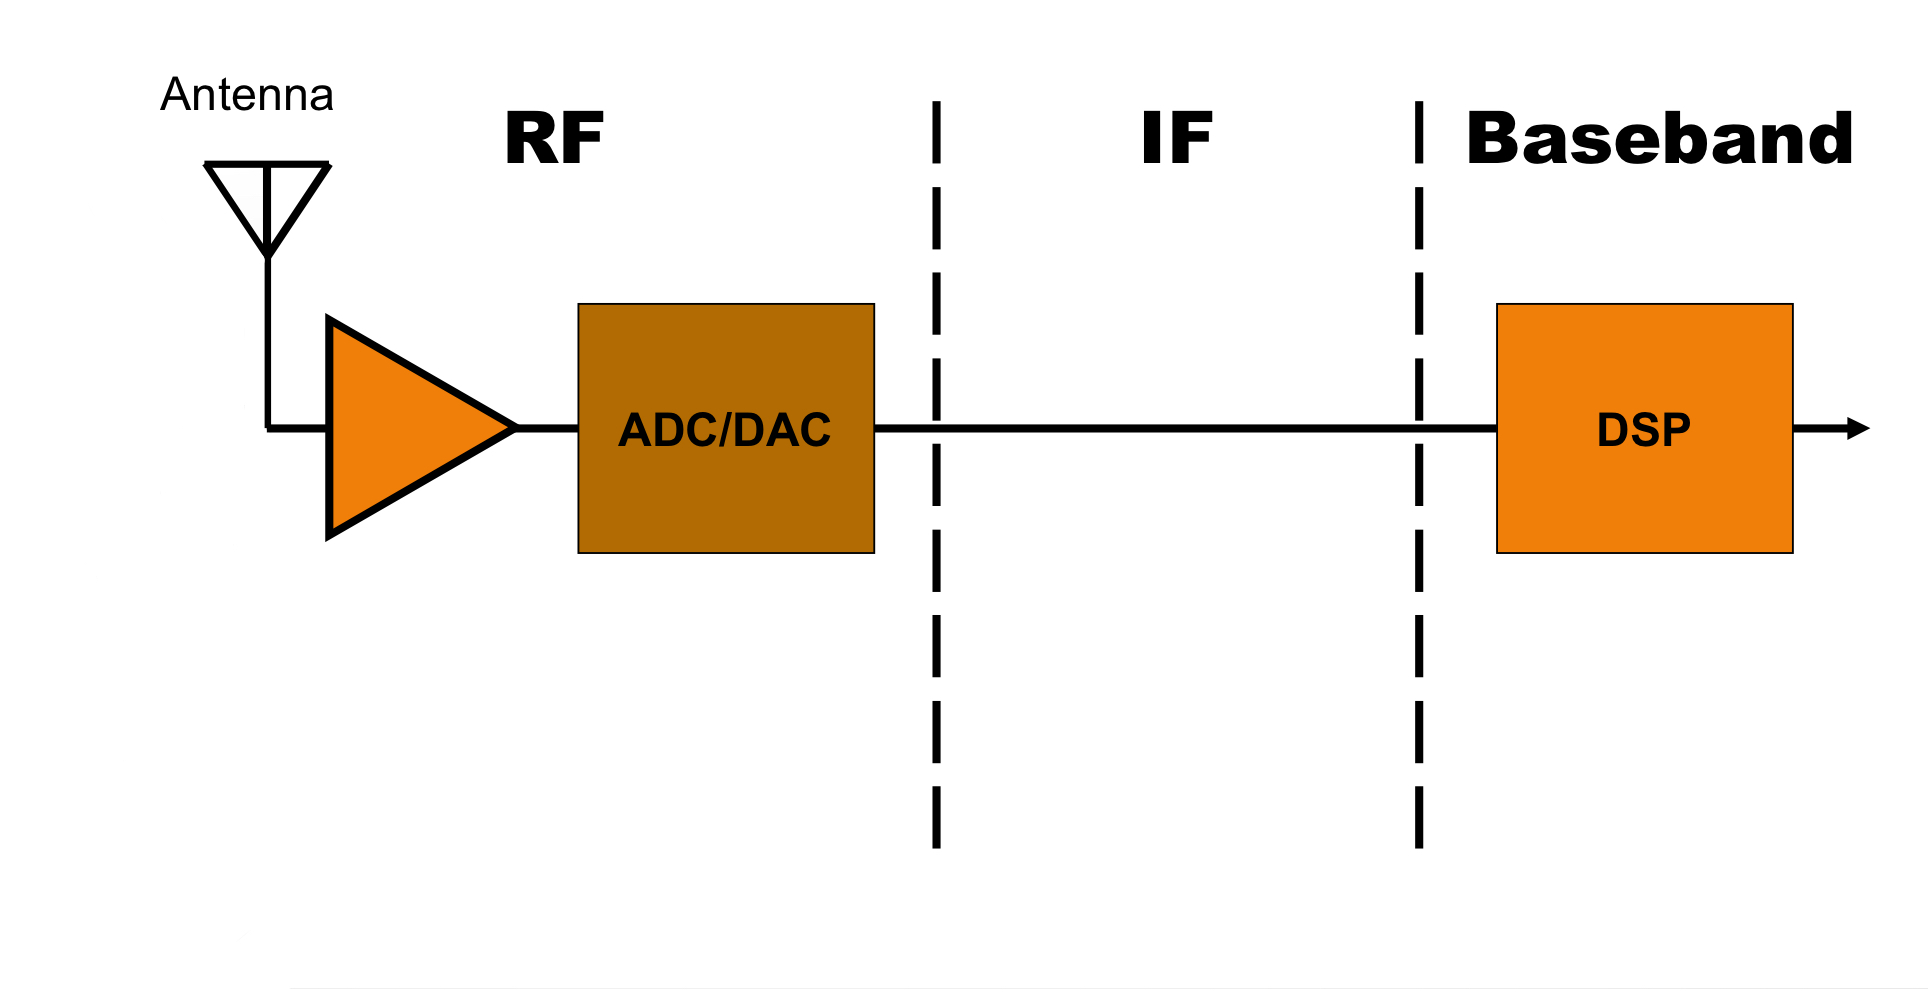
\includegraphics[width = 12cm]{imagenes/sdr.jpg}
 \caption{Software Defined Radio}
 \label{SDR}
 \end{figure}

Directamente se muestrea y se genera la señal en radio frecuencia (RF). Se consigue eliminar la inclusión de componentes en una frecuencia intermedia y se gana en flexibilidad, ya que todo el procedimiento se realiza en el dominio digital. También se obtiene una información más precisa al eliminar posibles mezcladores.

	 En concreto, el dispositivo RTL-SDR es un tipo de radio definida por software a la que se incorpora el chip ''RTL832U''. Este dispositivo es capaz de proporcionar las partes real y compleja de la señal en banda base, pudiendo abarcar gran parte del espectro de radio frecuencia. El sintonizador interno cubre un ancho de banda desde los 25 MHz hasta casi los 2 MHz. La frecuencia máxima de muestreo en este caso se sitúa en $2.4 MHz$.
	 
	 \begin{figure}[!tbp]
  \begin{subfigure}[b]{0.49\textwidth}
    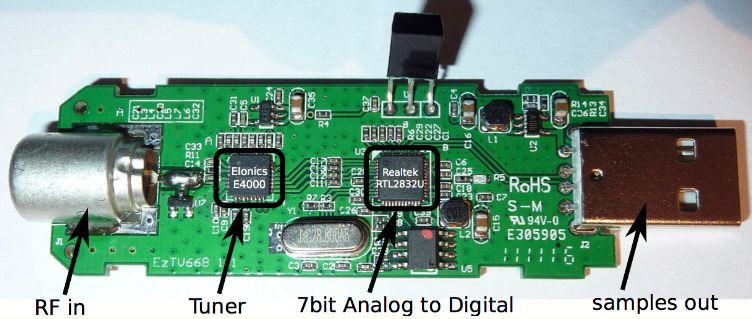
\includegraphics[width=\textwidth, height=5cm]{imagenes/inner_RTL.JPG}
    \caption{Interior RTL-SDR}
    \label{inner_RTL}
  \end{subfigure}
  \hfill
  \begin{subfigure}[b]{0.49\textwidth}
    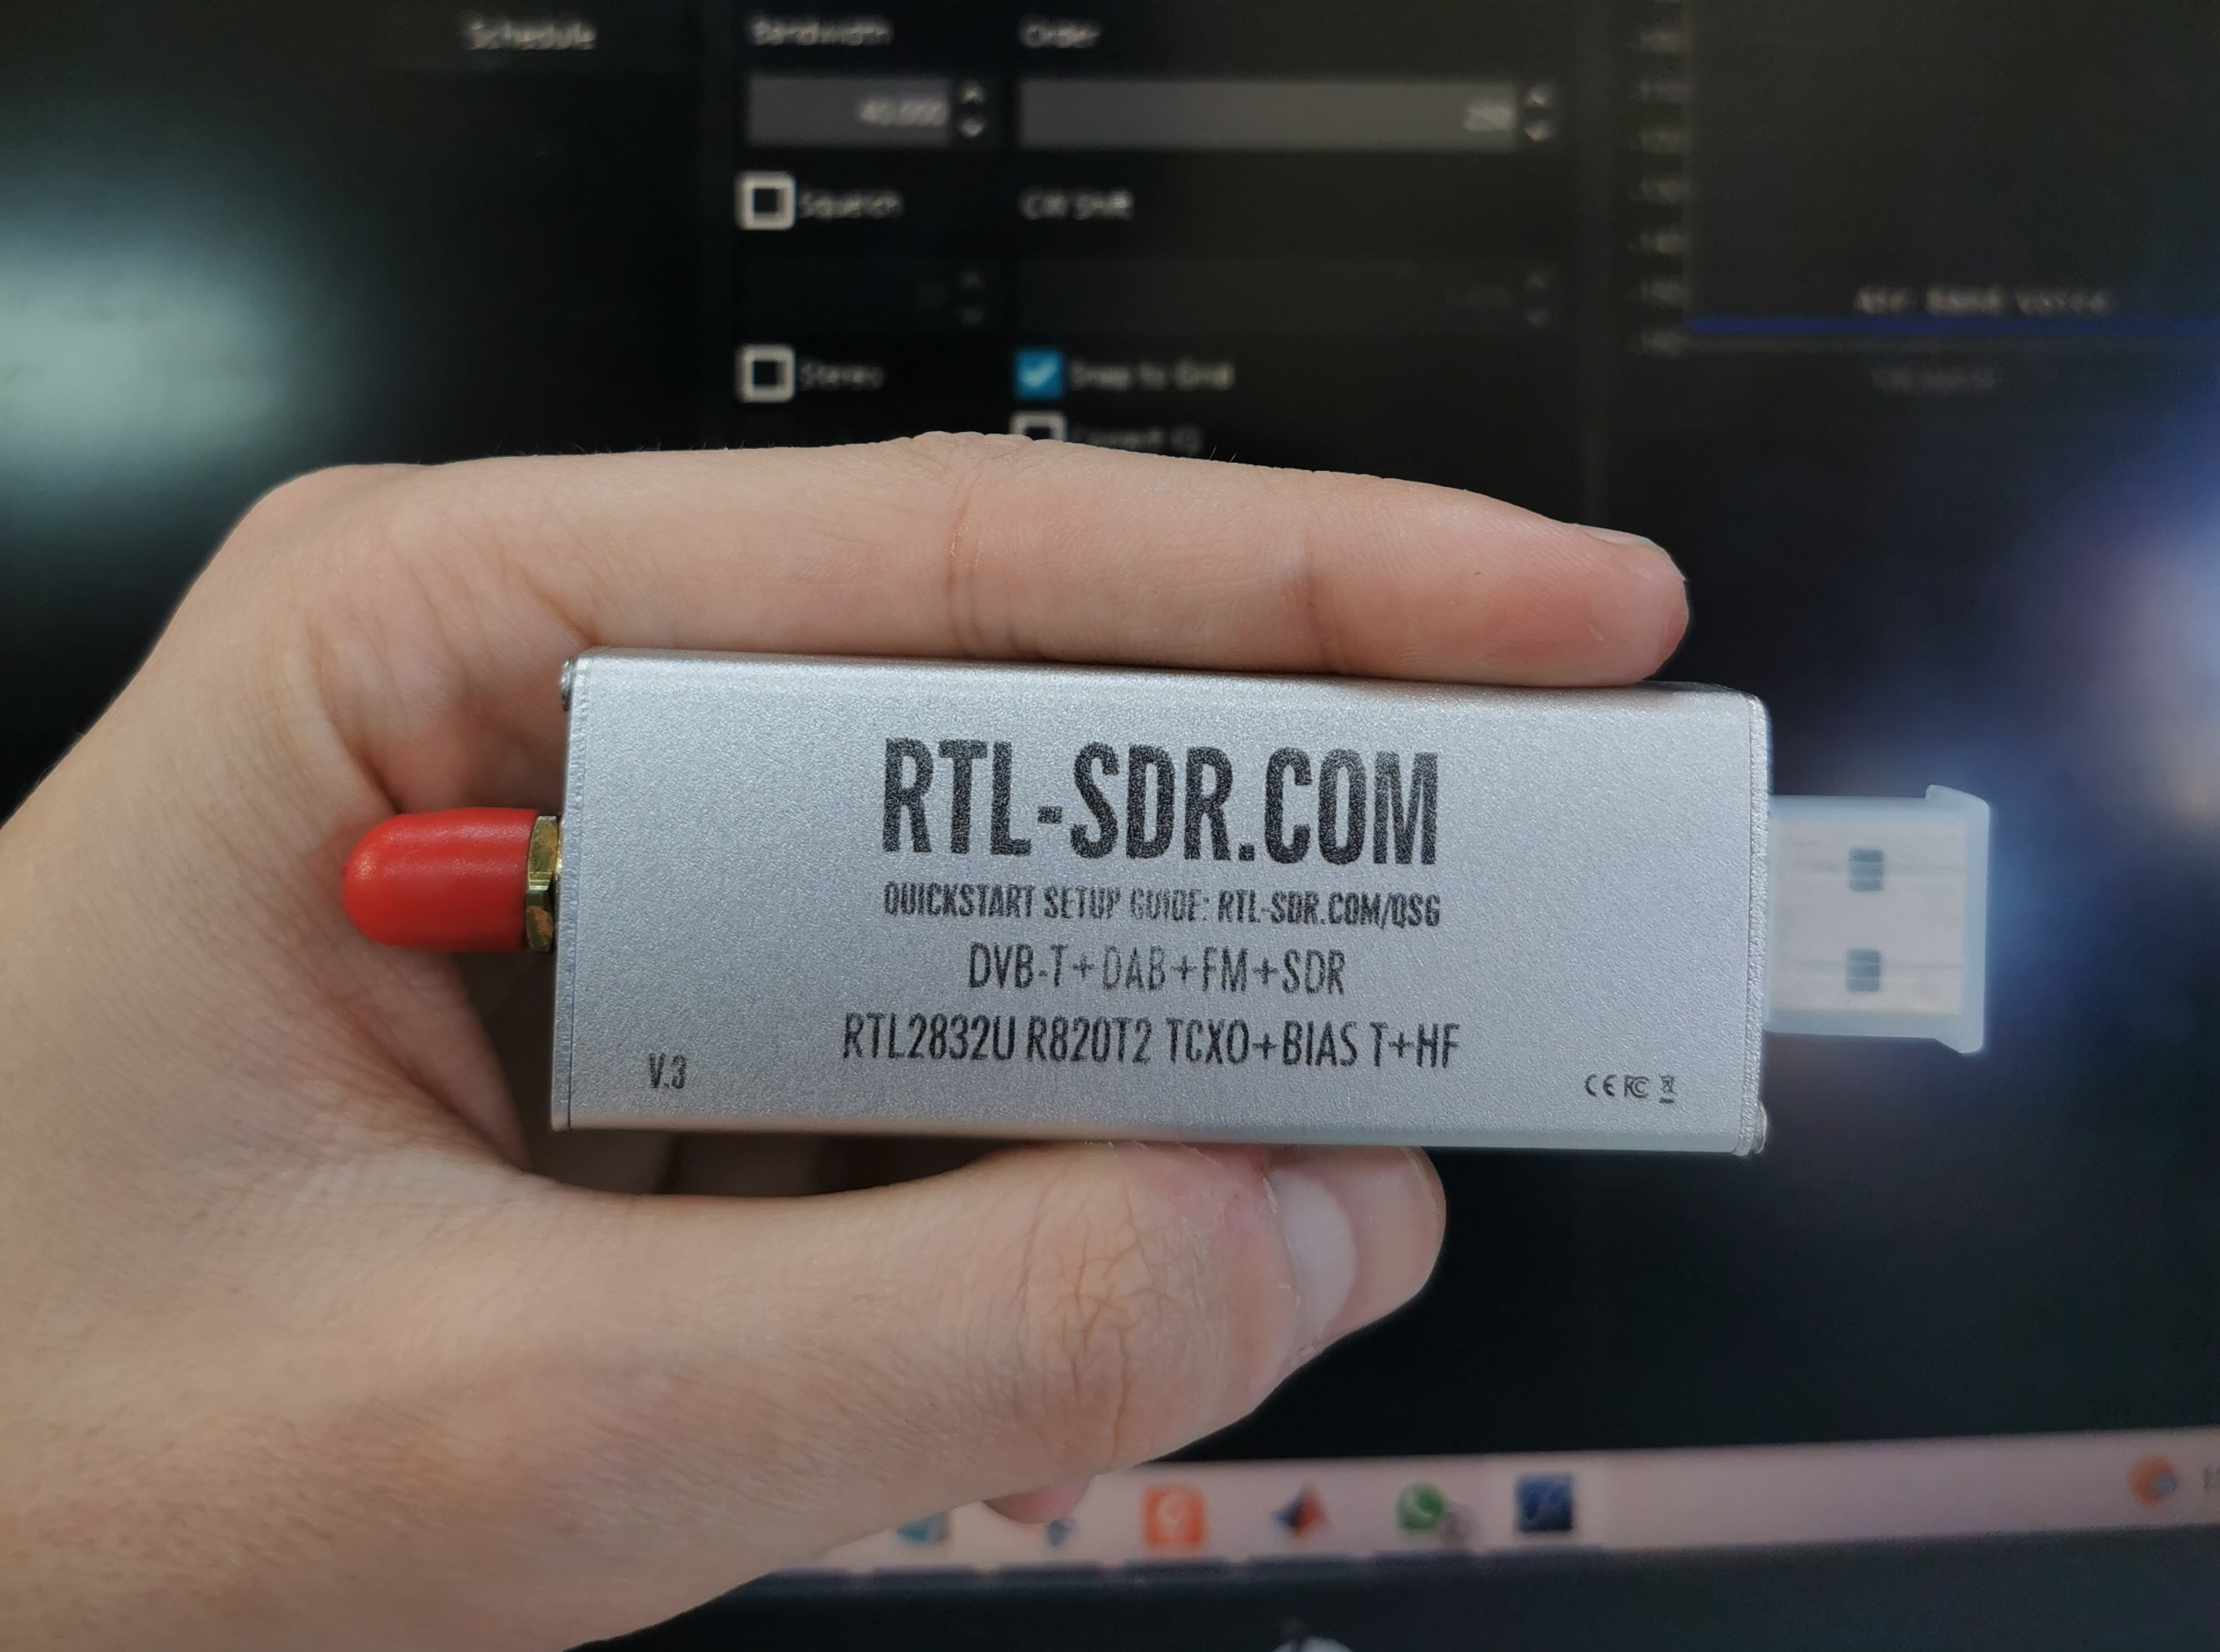
\includegraphics[width=\textwidth, height=5cm]{imagenes/rtl.JPG}
    \caption{RTL-SDR utilizado}
    \label{rtl}
  \end{subfigure}
  \caption{Esquema RTL-SDR}
\end{figure}

Este tipo de dispositivos fueron pensados primeramente como receptores DVB-T para la televisión, pero su gran versatilidad ha dado lugar a diferentes usos en FM, AM e incluso GPS.
El RTL-SDR utilizado en el proyecto se muestra en la \textit{Figura \ref{rtl}} y su interior en la \textit{Figura \ref{inner_RTL}.} 
\newpage
\section{Software}

	\subsection{Programa Gpredict}
	Se ha utilizado como herramienta de apoyo el programa \textit{Gpredict}. Es un programa que llega a proporcionar información sobre una gran cantidad de satélites, así como su órbita, velocidad y frecuencia a la que emiten, tiempo en función de la posición...
	
	Es necesario definir primero una estación baso. En el caso de este proyecto, se han definido las coordenadas de Granada, España. Una vez definida la estación base, se seleccionan los satélites a los que les quieres realizar el seguimiento. En este caso serán los satélites NOAA activos (NOAA-18, NOAA-19 y NOAA-15). La interfaz del programa con la estación base y los satélites definidos se muestra en la \textit{Figura \ref{gpredict}}.
	
	\begin{figure}[hbtp]
 \centering
 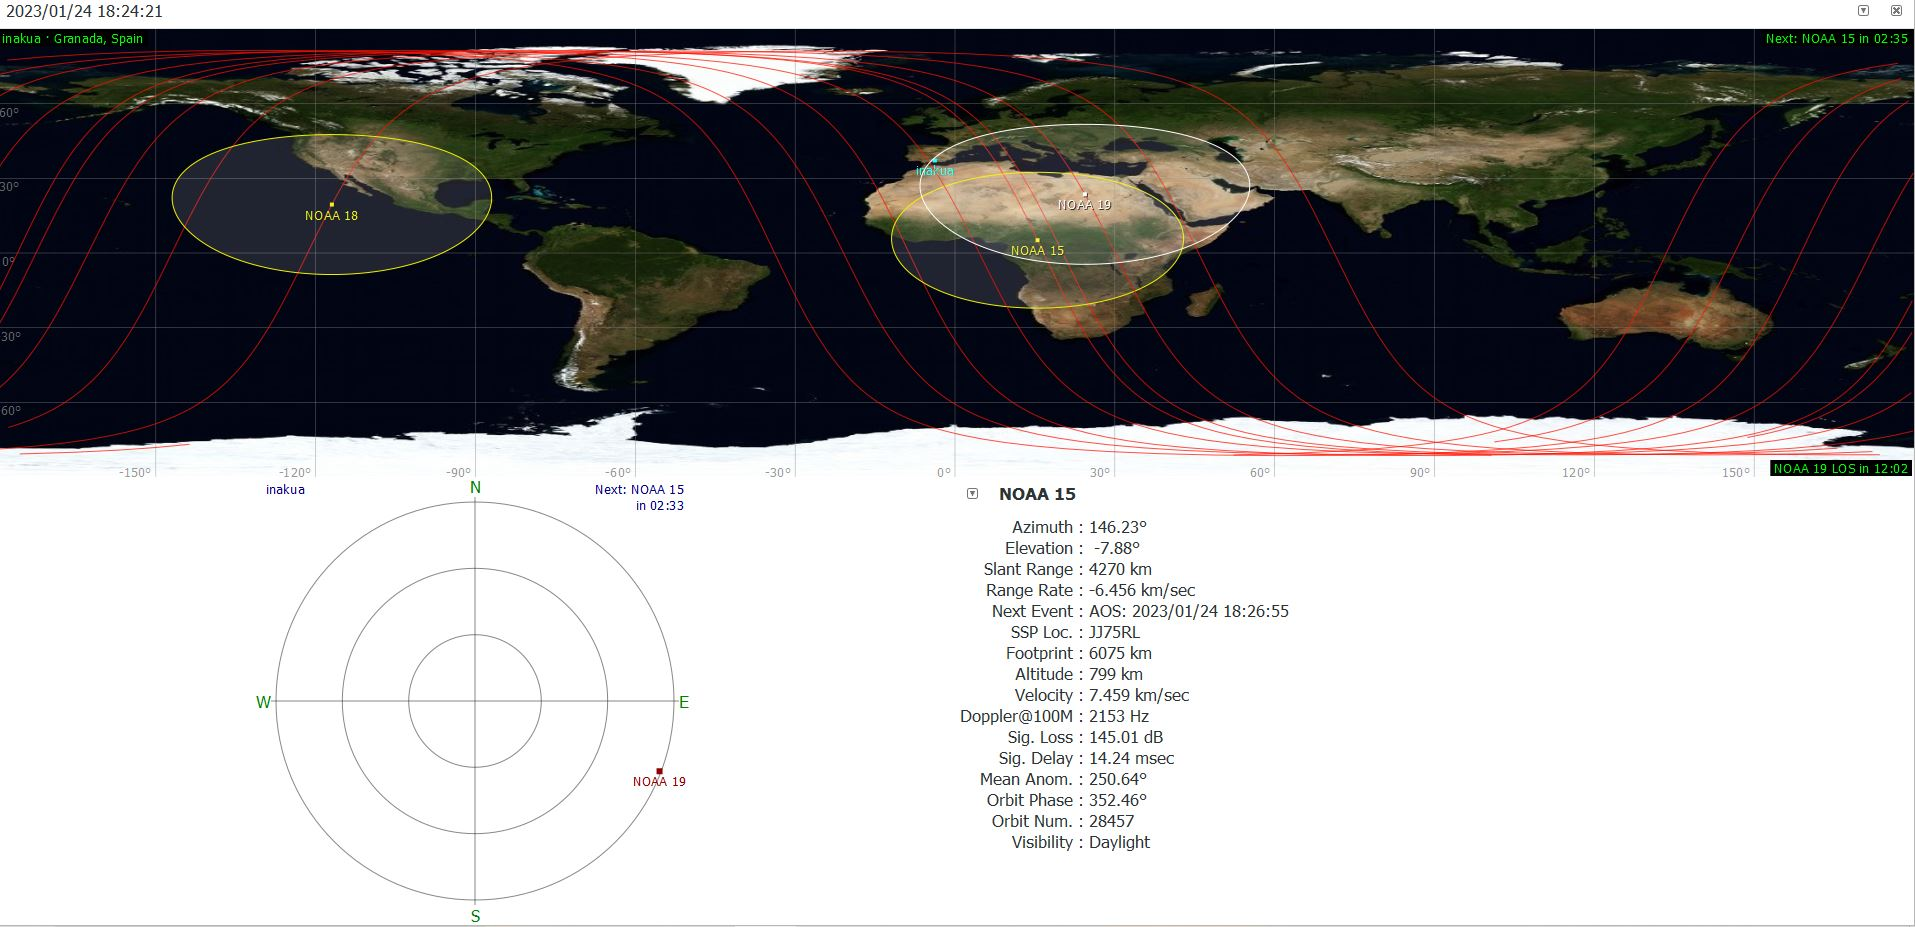
\includegraphics[width = 16cm]{imagenes/Gpredict_NOAA.JPG}
 \caption{Gpredict satélites NOAA}
 \label{gpredict}
 \end{figure}
 
 En la parte inferior de la captura de pantalla se puede visualizar la posición en coordenadas del satélite y otros datos como la velocidad, altitud, fase, elevación y hasta una aproximación del efecto Doppler en unidades de frecuencia.
 
 Más información sobre cada satélite se puede consultar mediante click derecho en el satélite en cuestión. Es de interés la información de \textit{Future Passes}, la cual ayuda a saber a qué momento del día va a pasar el satélite cerca de nuestra ubicación de la estación base.

	\begin{figure}[hbtp]
 \centering
 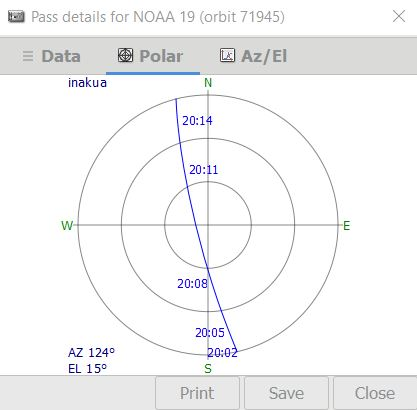
\includegraphics[width = 9cm]{imagenes/future_passes.JPG}
 \caption{Trayectoria NOAA-19}
 \label{trayectoria}
 \end{figure}
 
 
  Dentro de esta misma opción, se puede visualizar gráficamente la trayectoria del satélite, como se observa en la \textit{Figura \ref{trayectoria}}. Esta representación es de gran ayuda para saber el tiempo óptimo a la hora de captar la señal. Con los datos proporcionados por \textit{Gpredict}, se ha logrado en este proyecto captar las señales de los satélites NOAA para los tiempos previstos, por lo que es de gran utilidad.

	\subsection{Diagrama de flujo en GNU Radio}
	Con el propósito de procesar la señal recibida del RTL-SDR a tiempo real se ha creado un diagrama de bloques en GNU Radio. Los pasos a realizar en el procesamiento de la señal se han realizado teniendo en cuenta el estándar APT y son los siguientes:
	\begin{enumerate}
	\item Filtrado paso baja y decimado
	
		\begin{figure}[hbtp]
 \centering
 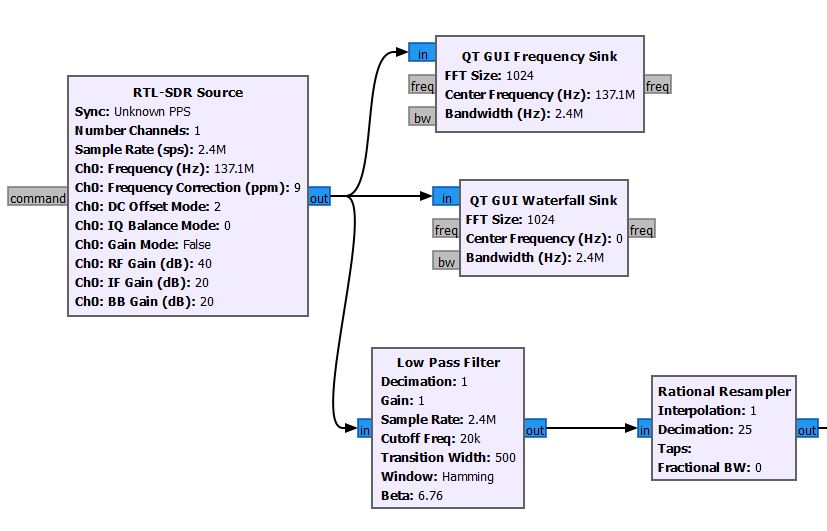
\includegraphics[width = 12cm]{imagenes/primer_paso.JPG}
 \caption{Filtrado y decimado}
 \label{filtardo_decimado}
 \end{figure}
 
 El bloque de ''RTL-SDR Source'' capta la señal directamente del dispositivo, con una tasa de muestreo de $2.4 MHz$, la frecuencia central la del satélite deseado y una ganancia en RF bastante alta (unos 35-40 dB).
 Se filtra paso baja con una frecuencia de corte poco restrictiva de $20 kHz$ para eliminar contribuciones ruidosas, ya que debido al efecto doppler, la frecuencia central de la señal del satélite podría variar y si se posee un ancho de banda restrictivo parte de la información podría perderse. Posteriormente se remuestrea la señal para trabajar a $96 kHz$.

Los bloques restantes no mencionados corresponden a \textit{GUI }, es decir, el espectro de la señal mostrado por pantalla.
 
 
 
	\item Demodulación FM
	
		\begin{figure}[hbtp]
 \centering
 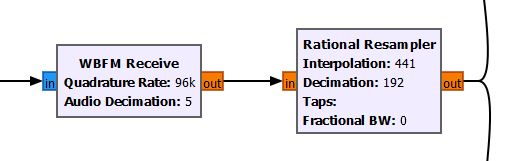
\includegraphics[width = 12cm]{imagenes/wbfm.JPG}
 \caption{Demodulación FM}
 \label{wbfm}
 \end{figure}
 
 Para demodular en FM simplemente se ha utilizado el bloque \textit{WBFM} el cual demodula la señal FM de banda ancha de entrada. Una vez con la señal demodulada, se adapta la frecuencia de muestreo a una típica de audio.	
	
	\item Demodulación AM y construcción de la imagen
	
		\begin{figure}[hbtp]
 \centering
 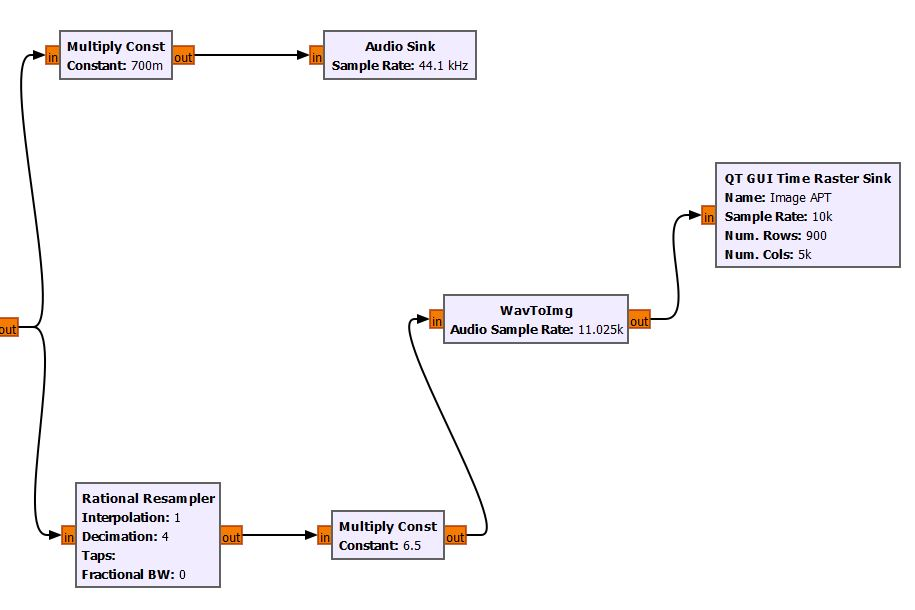
\includegraphics[width = 12cm]{imagenes/apt_blocks.JPG}
 \caption{Demodulación AM}
 \label{apt_blocks}
 \end{figure}
	
	
Después de obtener la señal de audio a la frecuencia de $11.025 kHz$, se llega a un bloque jerárquico llamado \textit{WavToImg} el cual realiza la correspondiente conversión de señal de audio a imagen APT. El interior de este bloque se muestra en la \textit{Figura \ref{wavtoimage}}.

 \begin{figure}[hbtp]
 \centering
 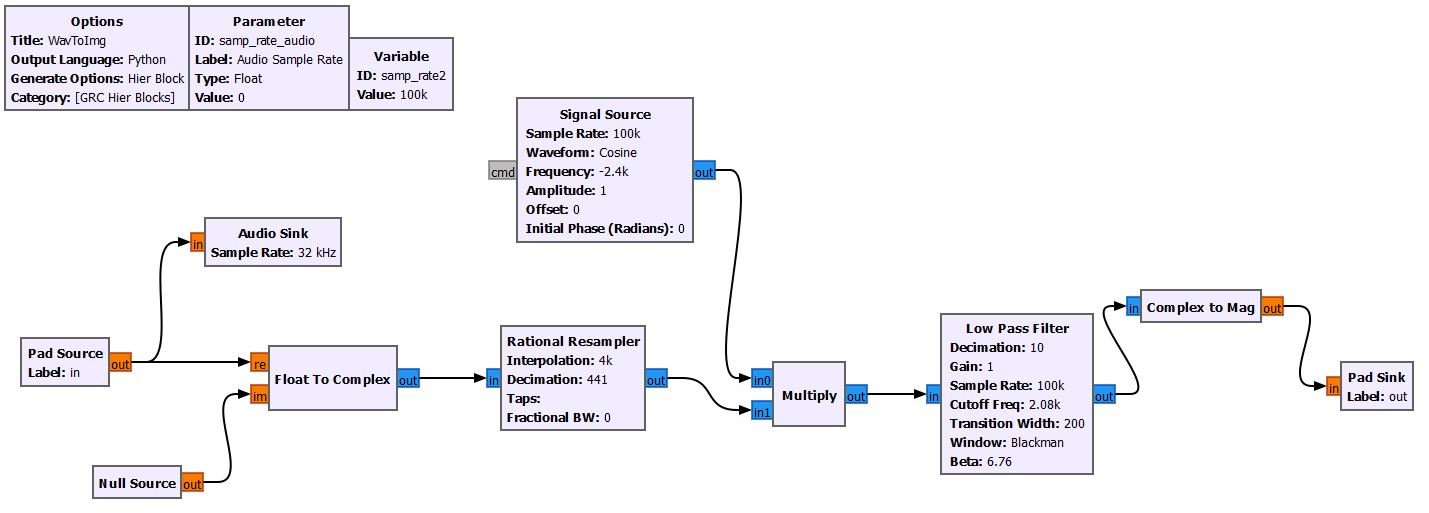
\includegraphics[width = 17cm]{imagenes/APT_hier.JPG}
 \caption{Bloque WavToImg}
 \label{wavtoimage}
 \end{figure}	
 
 El procedimiento se basa en una demodulación AM teniendo en cuenta que la información APT de interés se encuentra en una subportadora de $2.4 kHz$. 
	Según el estándar, se recomienda hacer un remuestreo a una frecuencias e $100 kHz$ antes de hacer la demodulación. Para llevar la subportadora a banda base se ha utilizado un coseno a una frecuencia de $-2.4 kHz$ y se ha hecho un filtrado posterior.
	
La salida del bloque "WavtoImg" proporciona la señal APT demodulada y se muestra la imagen por pantalla a tiempo real.
	
	
	\end{enumerate}
	
	 En la \textit{Figura \ref{diagrama_completo}} se aprecia el diagrama de flujo completo.
	
	\begin{figure}[hbtp]
 \centering
 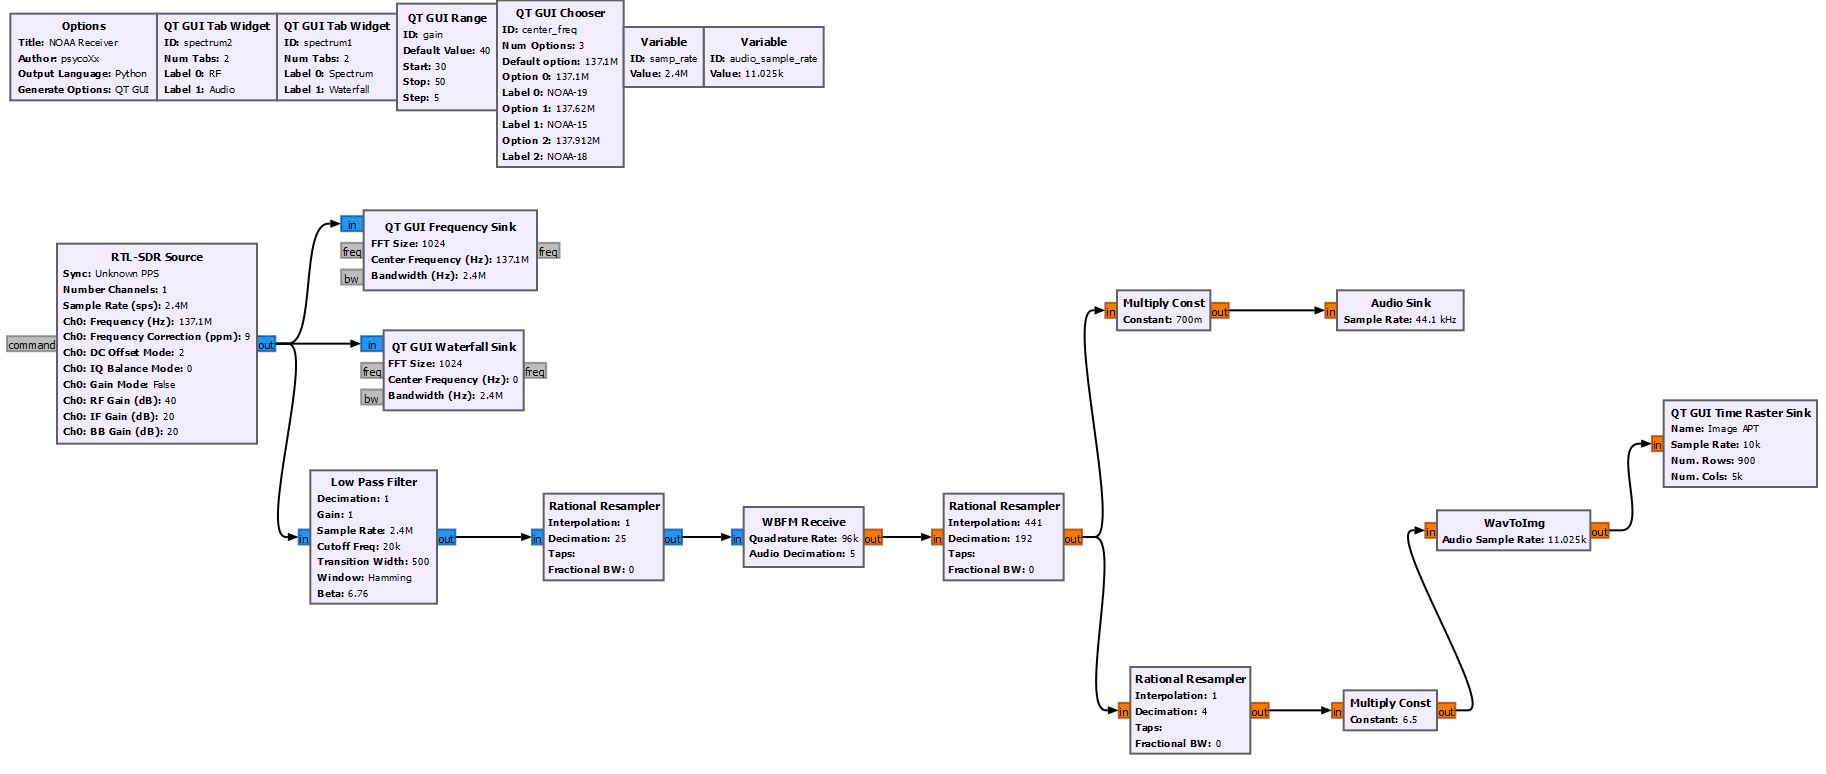
\includegraphics[width = 17cm]{imagenes/diagrama_flujo_completo.JPG}
 \caption{Diagrama de flujo}
 \label{diagrama_completo}
 \end{figure}




	\subsection{Corrección del efecto Doppler}

\section{Resultados}

\section{Dificultades en la realización del proyecto}

\newpage
\section{Conclusiones y líneas futuras}

Este proyecto se ha realizado durante dos meses y con una disponibilidad temporal de los integrantes limitada. A pesar de ello, se ha logrado avanzar relativamente rápido y se han logrado unos buenos resultados. Ha sido un proyecto con poco presupuesto, por lo que, seguramente, invirtiendo en una antena con mejores prestaciones o la incorporación de un empotrado hubiera mejorado notablemente los resultados.
Ha sido un proyecto bastante completo, ya que se ha profundizado en diseño de antenas, a la hora de construir la antena de tipo dipolo en V y en el procesado de señal con la parte de radio definida por software. Además, los objetivos iniciales del proyecto se han abarcado sin problemas, ya que se ha logrado captar correctamente múltiples señales de satélites NOAA convirtiendo estas a imágenes perfectamente visibles, consiguiendo una corrección del efecto Doppler muy precisa.

Como futuras mejoras, se propone la construcción de una antena con polarización circular, ya que esta es independiente de la orientación y no haría falta un factor externo para optimizar la captación de la señal a medida que el satélite se desplaza. 
Otra mejora sería la inclusión de un sistema empotrado conectado al RTL-SDR. De esta manera, mediante alguna orden externa, se podría captar la señal sin la necesidad de tener conectado un hardware como puede ser el ordenador.
Respecto a la corrección del efecto doppler, se ha propuesto una vía alternativa mediante la regresión lineal, la cual no depende de datos como la velocidad del satélite. Sin embargo, esta corrección que se ha realizado se realiza de forma asíncrona, por lo que una nueva mejora sería implementar una corrección del efecto doppler a tiempo real. De esta nueva forma serán necesarios datos como la velocidad del satélite en todo momento y la debida conexión a un software de seguimiento de satélites a tiempo real como puede ser \textit{Gpredict}.



\end{document}
